\documentclass[aspectratio=169,11pt]{beamer}

% ---------- plain custom style ----------
\usepackage{booktabs}
\usepackage{array}
\usepackage{graphicx}
\graphicspath{{../paper/figures/}}
\definecolor{accent}{HTML}{0072B2}
\definecolor{warm}{HTML}{D55E00}
\definecolor{ink}{HTML}{1F2328}
\definecolor{muted}{HTML}{6B7280}
\setbeamercolor{normal text}{fg=ink,bg=white}
\setbeamercolor{frametitle}{fg=ink,bg=white}
\setbeamercolor{title}{fg=ink}
\setbeamercolor{structure}{fg=accent}
\setbeamercolor{alerted text}{fg=warm}
\setbeamerfont{frametitle}{size=\Large,series=\bfseries}
\setbeamertemplate{navigation symbols}{}
\setbeamertemplate{itemize items}{\small\raise0.3ex\hbox{$\bullet$}}
\setbeamertemplate{frametitle}{\vspace{0.6em}\insertframetitle\par\vspace{0.15em}{\color{accent}\rule{2.2em}{2pt}}}
\setbeamertemplate{footline}{\hfill{\color{muted}\scriptsize\insertframenumber\ /\ \inserttotalframenumber}\hspace{1.2em}\vspace{0.8em}}
\newcommand{\hl}[1]{{\color{accent}\bfseries #1}}
\newcommand{\subtle}[1]{{\color{muted}\small #1}}

\title{How Far Do Hand-Built Linguistic Features Go?}
\subtitle{Reading-level classification on OneStopEnglish under article-grouped evaluation}
\author{Mohammed Alkhatib \and Alpartun Gunhan \and Jason Legarda}
\institute{Group 23}
\date{}

\begin{document}

% 1
\begin{frame}[plain]
\vspace{2.5em}
{\color{accent}\rule{3em}{3pt}}\par\vspace{0.8em}
{\huge\bfseries How far do hand-built\\[0.2em] linguistic features go?\par}
\vspace{0.8em}
{\large Reading-level classification on OneStopEnglish\\under article-grouped evaluation\par}
\vspace{2em}
{\color{muted} Mohammed Alkhatib \quad Alpartun Gunhan \quad Jason Legarda \quad --- \quad Group 23}
\end{frame}

% 2
\begin{frame}{The question}
\begin{columns}[T]
\column{0.55\textwidth}
Can linguistic features \textbf{we implement ourselves} label a news text as
\textbf{elementary}, \textbf{intermediate} or \textbf{advanced} better than a readability formula?
\vspace{1em}
\begin{itemize}
\item How much better than \textbf{Flesch-Kincaid}?
\item Which \textbf{feature group} carries the signal?
\item Which levels get \textbf{confused}, and why?
\item Extension: \textbf{pairwise ranking} (which of two texts is harder?)
\end{itemize}
\column{0.4\textwidth}
\vspace{0.5em}
\textbf{OneStopEnglish}\\
\subtle{Vajjala \& Lučić, 2018}\par\vspace{0.6em}
189 Guardian articles\\
$\times$ 3 versions rewritten by teachers\\
= \hl{567 texts}, 189 per level
\end{columns}
\end{frame}

% 3
\begin{frame}{We found two problems in the public corpus}
\begin{columns}[T]
\column{0.5\textwidth}
\textbf{1. Intermediate files lost their punctuation}\par\vspace{0.4em}
\small
{\color{muted}Damaged:}\quad \emph{Our guardian angel will take care of you, said mission control}\par\vspace{0.2em}
{\color{muted}Intact:}\quad\ \ \emph{{\color{accent}\textbf{``}}Our guardian angel will take care of you,{\color{accent}\textbf{''}} said mission control}\par\vspace{0.6em}
\normalsize
Every curly quote, apostrophe, \pounds{} and \'e is deleted --- only in the intermediate files.\\
\alert{A model can spot ``intermediate'' from punctuation alone.}\par\vspace{0.3em}
\subtle{Fix: an intact copy hides in a nested folder.}
\column{0.45\textwidth}
\textbf{2. One text is a duplicate}\par\vspace{0.4em}
\texttt{Royal Baby-ele.txt} is byte-identical to \texttt{Skydiver-ele.txt}.\par\vspace{0.3em}
\subtle{Fix: rebuilt from the authors' CSV export.}
\vspace{1.4em}

\textbf{Splits by article, not by text}\par\vspace{0.4em}
All 3 versions of an article stay together.\\
\hl{38 articles} held out as test (used once);\\
\hl{151 articles} in 5 grouped CV folds.
\end{columns}
\end{frame}

% 4
\begin{frame}{Five systems, 27 features}
\begin{columns}[T]
\column{0.38\textwidth}
\begin{enumerate}
\item Majority class
\item Length only (word count)
\item Flesch-Kincaid (computed ourselves)
\item \textbf{Feature logistic regression} \subtle{(main)}
\item Character n-gram SVM \subtle{(strong comparison)}
\end{enumerate}
\vspace{0.6em}
\subtle{Baselines 2--3: two cut-offs learned on training folds. C tuned by inner grouped CV. 95\% CIs: bootstrap over articles.}
\column{0.6\textwidth}
\footnotesize
\begin{tabular}{@{}l>{\raggedright\arraybackslash}p{4.9cm}@{}}
\toprule
\textbf{Group} & \textbf{Examples} \\
\midrule
Word length (3) & syllables/word, \% 3+ syllables \\
Sentence length (3) & mean, max, SD words/sentence \\
Vocabulary (3) & \% outside top 3,000 words; Zipf freq. \\
Lexical variation (8) & TTR (100 words); POS ratios \\
Syntax (5) & parse depth; subordinate clauses; passives \\
Discourse (5) & connectives per sentence \\
\bottomrule
\end{tabular}
\end{columns}
\end{frame}

% 5
\begin{frame}{Results: features beat the formula by 14--20 points}
\centering
\begin{tabular}{lcc}
\toprule
System & Dev CV & \textbf{Test} [95\% CI] \\
\midrule
Majority class & 33.3 & 33.3 \\
Flesch-Kincaid & 51.7 & 56.1 [48.2, 64.0] \\
Length only & 62.3 & 64.0 [57.0, 70.2] \\
{\color{accent}\textbf{Feature LR (ours)}} & {\color{accent}\textbf{71.3}} & {\color{accent}\textbf{70.2 [62.3, 78.1]}} \\
Char n-gram SVM & 73.3 & 73.7 [68.4, 79.0] \\
Feature LR + word count & 77.7 & 78.9 [70.2, 86.8] \\
\bottomrule
\end{tabular}
\vspace{1em}

\raggedright
\begin{itemize}
\item Ours vs.\ Flesch-Kincaid: \textbf{+14.0 points on test} [3.5, 24.6]
\item \textbf{Word count beats Flesch-Kincaid}: editors cut content for lower levels
\item Ours $\approx$ char SVM, but the SVM rarely predicts intermediate (11/38 vs.\ 21/38)
\end{itemize}
\end{frame}

% 6
\begin{frame}{Which features carry the signal?}
\centering
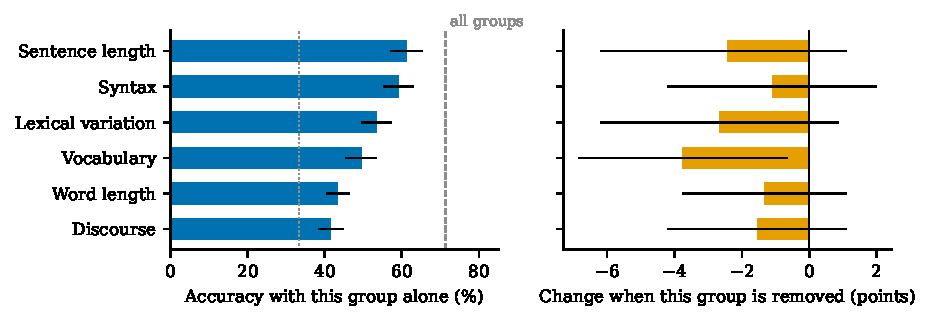
\includegraphics[width=0.82\textwidth]{ablation.pdf}
\vspace{0.3em}
\raggedright
\begin{itemize}
\item \textbf{Sentence length} (61\%) and \textbf{syntax} (59\%) are strongest alone
\item Groups overlap, so removing one costs little --- except \textbf{vocabulary} ($-$3.8, CI excludes 0)
\item Word length adds almost nothing once word frequency is known
\end{itemize}
\end{frame}

% 7
\begin{frame}{Surprise: sharing articles across folds \emph{lowers} accuracy}
\begin{columns}[c]
\column{0.5\textwidth}
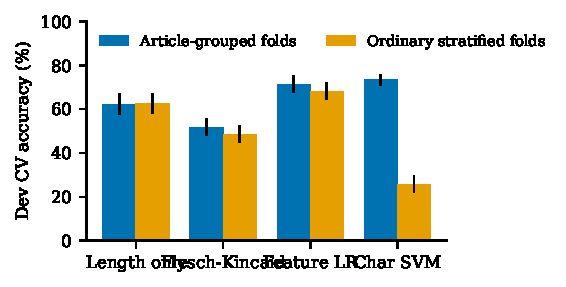
\includegraphics[width=\textwidth]{splitcheck.pdf}
\column{0.47\textwidth}
We expected ordinary stratified folds to \textbf{inflate} scores.\par\vspace{0.6em}
Instead the char SVM falls to \alert{\textbf{25.8\%}} --- below chance.\par\vspace{0.6em}
\textbf{Why:} an article's other versions always have a \emph{different} label. Recognise the article $\Rightarrow$ copy a wrong label.\par\vspace{0.6em}
\subtle{98\% of the SVM's errors predict the label of a sibling it saw in training.}
\end{columns}
\end{frame}

% 8
\begin{frame}{Pairwise ranking: easy within an article, not across}
\centering
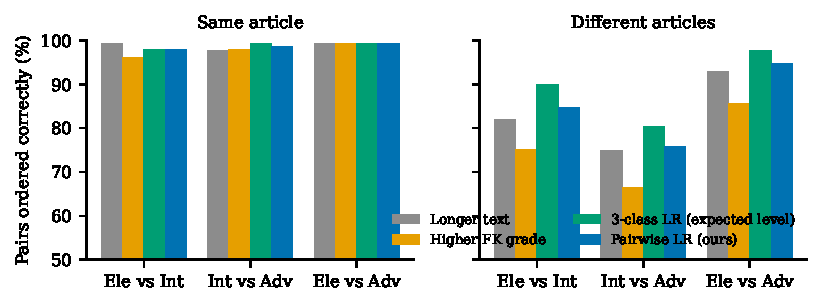
\includegraphics[width=0.8\textwidth]{ranking.pdf}
\vspace{0.2em}
\raggedright
\begin{itemize}
\item Same article: \textbf{$\sim$99\% for everything}, even ``the longer text is harder'' (100\% on test)
\item Different articles: methods separate --- 3-class model 89\%, our pairwise ranker 85\%, length 83\%
\end{itemize}
\end{frame}

% 9
\begin{frame}{Errors: intermediate, and articles that are just harder}
\begin{columns}[c]
\column{0.52\textwidth}
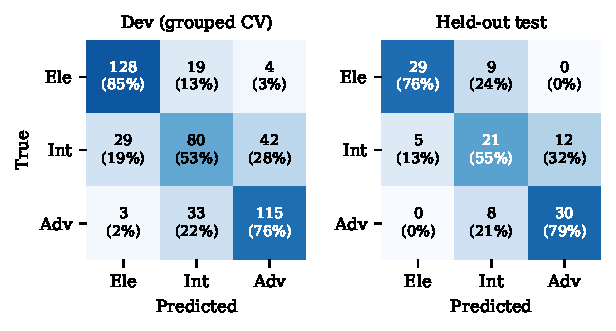
\includegraphics[width=\textwidth]{confusion.pdf}
\column{0.45\textwidth}
\textbf{95\%} of errors involve intermediate; elementary vs.\ advanced: 7 on dev, 0 on test.\par\vspace{0.7em}
\textbf{Levels are relative to the article.}\\
\hl{61\%} of Flesch-Kincaid variance is between articles, only \hl{31\%} between levels.\par\vspace{0.5em}
\subtle{\emph{Switched Babies} (advanced, grade 9.0) $\rightarrow$ predicted intermediate.\\
\emph{Violence} report (intermediate, grade 12.2) $\rightarrow$ predicted advanced.}
\end{columns}
\end{frame}

% 10
\begin{frame}{Takeaways}
\begin{enumerate}
\setlength\itemsep{0.7em}
\item 27 interpretable features: \textbf{70--71\%}, \textbf{+14--20 points over Flesch-Kincaid}, on a par with char n-grams.
\item \textbf{Sentence length and syntax} carry most signal; \textbf{word frequency} is the one group you can't drop.
\item On parallel corpora, shared articles across folds \textbf{deflate} accuracy --- the opposite of what we expected.
\item Ordering versions of one article is \textbf{trivial}; the hard part is \textbf{absolute} level across stories.
\item Check the data: the public release \textbf{leaks the label} through stripped punctuation.
\end{enumerate}
\end{frame}

% 11
\begin{frame}{Limitations}
\begin{itemize}
\setlength\itemsep{0.6em}
\item One corpus; test set of 38 articles $\Rightarrow$ CIs about $\pm$8 points
\item CLEAR cross-corpus test planned but not run
\item spaCy small model parses not checked by hand; our own connective list
\item Prior-work numbers use different protocols --- reference points, not benchmarks
\end{itemize}
\vfill
\centering
{\Large\bfseries Thank you --- questions?}\par\vspace{0.4em}
\subtle{Code, cleaned data and paper: github.com/MohdAlkhatib/nlp}
\end{frame}

\end{document}
